\documentclass[english, aspectratio=169]{beamer}
% english is for the language used in standard texts (figures, tables etc)
% aspectratio of 16:9 or set it for more old school to 4:3 (without the ':')

% ---------------------------------------------------------------------------- %
% Load base preamble
% ---------------------------------------------------------------------------- %
\usepackage{import}
\subimport{../preamble/}{beamer.tex}

% ---------------------------------------------------------------------------- %
% Local settings
% ---------------------------------------------------------------------------- %
\newcommand{\B}[0]{\ensuremath{\mathbb{B}}}

\newcommand{\sort}[0]{\text{sort}}

\newcommand{\triple}[3]{\ensuremath{(#1, #2, #3)}}
\renewcommand{\arc}[3]{\ensuremath{#1 \xrightarrow{_{#2}} #3}}


\tikzstyle{plot_adiar}=[color=black, mark=o, mark size=1pt, line width=0.7pt]
\tikzstyle{plot_buddy}=[color=red, mark=o, mark size=1pt, line width=0.7pt]
\tikzstyle{plot_cudd}=[color=blue, mark=diamond, mark size=1pt, line width=0.7pt]
\tikzstyle{plot_sylvan}=[color=purple, mark=square, mark size=1pt, line width=0.7pt]

% Horizontal legends: https://tex.stackexchange.com/a/101578
% argument #1: any options
\makeatletter
\newenvironment{customlegend}[1][]{%
    \begingroup
    % inits/clears the lists (which might be populated from previous
    % axes):
    \pgfplots@init@cleared@structures
    \pgfplotsset{#1}%
}{%
    % draws the legend:
    \pgfplots@createlegend
    \endgroup
}%

% makes \addlegendimage available (typically only available within an
% axis environment):
\def\addlegendimage{\pgfplots@addlegendimage}
\makeatother

% ------------------------------------------------------------------------------
% TITLEPAGE
% ------------------------------------------------------------------------------
\title{
  Efficient External Memory Algorithms\\
  for Binary Decision Diagram Manipulation
}

\author{\textbf{Steffan Christ S\o lvsten},
  Jaco van de Pol,\\
  Anna Blume Jakobsen,
  and Mathias Weller Berg Thomasen
}

\institute{
\includegraphics[width=0.2\linewidth]{../external/aulogo_uk_var2_black.eps}}

\date{\today}

\begin{document}

\titleframe

\blankframe

\begin{frame}
  \begin{figure}
    \centering

    \begin{tikzpicture}
  % ALU
  \node[
  draw,
  trapezium,
  shape border rotate=180,
  text width=1cm,
  align=center,
  ] at (0.03,0) (cpu) {CPU};

  % Main memory
  \begin{scope}
    \clip(-1.13,1) rectangle (1.19,1.4);
    \filldraw[
    color=black!60!white,
    fill=black!5!white,
    pattern=vertical lines,
    pattern color=black!30!white
    ] (-9,1.25) rectangle ++(18,0.5)
    ;
  \end{scope}

  \node[
  draw,
  rectangle,
  text width=2.08cm,
  align=center,
  ] at (0.03,1.5) (m) {$M$};

  % Disk
  \begin{scope}
    \clip(-6,2.5) rectangle (6,2.9);
    \filldraw[
    color=black!60!white,
    fill=black!5!white,
    pattern=vertical lines,
    pattern color=black!30!white
    ] (-9,2.75) rectangle ++(18,0.5)
    ;
  \end{scope}

  \node[
  draw,
  rectangle,
  text width=5.04cm,
  align=center,
  ] at (0.03,3) (n) {$N$};

  \path[->]
  (cpu) edge[bend left=40] (m)
  (m) edge[bend left=40] (cpu)

  (n) edge[bend left=40] (m)
  (m) edge[bend left=40] (n)
  ;

  \node at (0.02,2.24) {\textcolor{gray}{$B$}};
\end{tikzpicture}


    \caption{The I/O model by Aggarwal and Vitter '87}
  \end{figure}

\end{frame}

\begin{frame}
  For any realistic values of $N$, $M$, and $B$ we have that

  \begin{equation*}
      N/B \quad < \quad \sort(N) \triangleq N/B \cdot \log_{M/B} N/B \quad \ll \quad N
    \enspace ,
  \end{equation*}

  \begin{theorem}[Aggarwal and Vitter '87]
    $N$ elements can be sorted in $\Theta(\sort(N))$ I/Os.
  \end{theorem}
  \begin{theorem}[Arge '95]
    $N$ elements can be inserted in and extracted from a Priority Queue in
    $\Theta(\sort(N))$ I/Os.
  \end{theorem}
\end{frame}

\blankframe

\begin{frame}
  %Representation of functions $\B^n \rightarrow \B$ by Bryant '86.

  \begin{figure}
    \centering

    \begin{subfigure}{0.49\linewidth}
      \centering

      \begin{tikzpicture}[scale=0.8, every node/.style={transform shape}]
          % nodes
  \node[shape = circle, draw = black]
  (0) {$x_0$};

  \node[shape = circle, draw = black, below right= .4cm and .5cm of 0]
  (1) {$x_1$};

  \node[shape = circle, draw = black, below left=.4cm and .5cm of 1]
  (2) {$x_2$};

  \node[shape = circle, draw = black, below left=.4cm and .5cm of 2]
  (31) {$x_3$};
  \node[shape = circle, draw = black, below right=.4cm and .5cm of 2]
  (32) {$x_3$};

  % leafs
  \node[shape = rectangle, draw = black, below=.4cm of 31]
  (sink_T) {$\top$};

  \node[shape = rectangle, draw = black, below=.4cm of 32]
  (sink_F) {$\bot$};

  % arcs
  \draw[->, dashed]
    (0)  edge (2)
    (1)  edge (2)
    (2)  edge (31)
    (31) edge (sink_T)
    (32) edge (sink_F)
  ;

  \draw[->]
    (0)  edge (1)
    (1)  edge (32)
    (2)  edge (32)
    (31) edge (sink_F)
    (32) edge (sink_T)
  ;
      \end{tikzpicture}

      \caption{$(x_0 \wedge x_1 \wedge x_3) \vee (x_2 \oplus x_3)$}
    \end{subfigure}
    \begin{subfigure}{0.49\linewidth}
      \centering

      \begin{tikzpicture}[scale=0.8, every node/.style={transform shape}]
          % nodes
  \node[shape = circle, draw = black]
  (0) {$x_0$};

  \node[shape = circle, draw = black, below left=1.4cm and .5cm of 0]
  (21) {$x_2$};

  \node[shape = circle, draw = black, below right=1.4cm and .5cm of 0]
  (22) {$x_2$};

  \node[shape = circle, draw = black, below right=0.4cm and .5cm of 21]
  (3) {$x_3$};

  % leafs
  \node[shape = rectangle, draw = black, below right=.4cm and .5cm of 3]
  (sink_F) {$\bot$};

  \node[shape = rectangle, draw = black, below left=.4cm and .5cm of 3]
  (sink_T) {$\top$};

  % arcs
  \draw[->, dashed]
    (0)  edge (21)
    (21) edge (sink_T)
    (22) edge (3)
    (3)  edge (sink_T)
  ;

  \draw[->]
    (0)  edge (22)
    (21) edge (3)
    (22) edge (sink_F)
    (3)  edge (sink_F)
  ;
      \end{tikzpicture}

      \caption{$\neg (x_0 \ ?\ x_2 \vee x_3 \ :\ x_2 \wedge x_3)$}
    \end{subfigure}

    \caption{Examples of (Reduced Ordered) Binary Decision Diagrams.}
  \end{figure}
\end{frame}

\begin{frame}
  \begin{theorem}[Bryant '86]
    For a fixed variable order, if one exhaustively applies the two rules below,
    then one obtains the Reduced OBDD, which is a unique canonical form of the
    function.    
  \end{theorem}

  \begin{figure}
    \centering
    
    \begin{subfigure}[b]{0.40\linewidth}
      \centering

      \begin{tikzpicture}[scale=0.9, every node/.style={transform shape}]
        \node[shape = circle, black, draw = black] (i) {$x_i$};
\node[shape = circle, draw = black, below=of i] (child) {};
\node[shape = circle, draw = black, above=of i] (parent) {};

% implication
\node[shape = circle, black,right=0.5cm of i] {$\implies$};

% after
\node[shape = circle, draw = black, right=2cm of child] (childafter) {};
\node[shape = circle, draw = black, right=2cm of parent] (parentafter) {};

\draw[->, dashed] (i) edge[bend right] (child);
\draw[->]
(i) edge[bend left] (child)
(parent) edge (i)
(parentafter) edge (childafter)
;

      \end{tikzpicture}

      \vspace{10pt}
      {\small {\bf (1)} Remove redundant nodes}
    \end{subfigure}
    \begin{subfigure}[b]{0.59\linewidth}
      \centering

      \begin{tikzpicture}[scale=0.9, every node/.style={transform shape}]
        \node[shape = circle, black, draw = black] (i1) {$x_i$};
\node[shape = circle, black, draw = black, right=of i1] (i2) {$x_i$};

\node[shape = circle, draw = black, below=of i1] (child1) {};
\node[shape = circle, draw = black, below=of i2] (child2) {};

\node[shape = circle, draw = black, above=of i1] (parent1) {};
\node[shape = circle, draw = black, above=of i2] (parent2) {};

% implication
\node[shape = circle, black,right=0.5cm of i2] {$\implies$};

% after
\node[shape = circle, draw = black, right=4cm of child1] (c1a) {};
\node[shape = circle, draw = black, right=4cm of child2] (c2a) {};

\node[shape = circle, black, draw = black, right=2.7cm of i2] (ia) {$x_i$};

\node[shape = circle, draw = black, right=4cm of parent1] (p1a) {};
\node[shape = circle, draw = black, right=4cm of parent2] (p2a) {};


\draw[->, dashed]
(i1) edge (child1)
(i2) edge (child1)
(ia) edge (c1a)
;
\draw[->]
(i1) edge (child2)
(i2) edge (child2)
(parent1) edge (i1)
(parent2) edge (i2)
(p1a) edge (ia)
(p2a) edge (ia)
(ia) edge (c2a)
;

      \end{tikzpicture}

      \vspace{10pt}
      {\small {\bf (2)} Merge duplicate nodes}
    \end{subfigure}

  \end{figure}
  
\end{frame}

\blankframe

\begin{frame}
  \begin{figure}
    \centering
    
    \begin{subfigure}[b]{0.48\linewidth}
      \centering

      \begin{tikzpicture}
        \begin{axis}[%
          width=0.95\linewidth, height=0.7\linewidth,
          every tick label/.append style={font=\scriptsize},
          % x-axis
          xlabel={number of nodes},
          xmajorgrids=true,
          xmin=800000 ,
          xmax=1200000000,
          xmode = log,
          % y-axis
          ymin=0.1,
          ymax=0.27,
          ylabel={$\mu$s / node},
          ytick distance={0.05},
          yminorgrids=false,
          ymajorgrids=true,
          grid style={dashed,black!20},
          ]

          \addplot [style=plot_buddy]
          table {./data/cache_buddy_time_per_node.tex};
        \end{axis}
      \end{tikzpicture}
    \end{subfigure}
    \quad
    \begin{subfigure}[b]{0.48\linewidth}
      \centering

      \begin{tikzpicture}
        \begin{axis}[%
          width=0.95\linewidth, height=0.7\linewidth,
          every tick label/.append style={font=\scriptsize},
          % x-axis
          xlabel={number of nodes},
          xmin=800000 ,
          xmax=1200000000,
          xmode = log,
          % y-axis
          ymin=2,
          ymax=5.95,
          ylabel={misses / node},
          ytick distance={1},
          yminorgrids=true,
          ymajorgrids=true,
          grid style={dashed,black!20},
          ]
          
          \addplot+ [style=plot_buddy]
          table {./data/cache_buddy_misses_per_node.tex};
        \end{axis}
      \end{tikzpicture}
    \end{subfigure}

    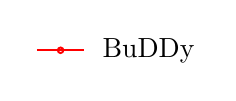
\begin{tikzpicture}
      \begin{customlegend}[
        legend columns=-1,
        legend style={draw=none,column sep=1ex},
        legend entries={BuDDy}
        ]
        \addlegendimage{style=plot_buddy}
      \end{customlegend}
    \end{tikzpicture}
    
    \caption{Cache behaviour for the $N$-Queens problem.}
  \end{figure}

\end{frame}

\begin{frame}
  \begin{figure}
    \centering
    
    \begin{tikzpicture}
      \begin{axis}[%
        width=0.69\linewidth, height=0.42\linewidth,
        every tick label/.append style={font=\scriptsize},
        % x-axis
        xlabel={Memory (GiB)},
        xmajorgrids=true,
        xmin=3.5,
        xmax=10.5,
        xtick={4, ..., 10},
        % y-axis
        ylabel={time (seconds)},
        yminorgrids=false,
        ymajorgrids=true,
        grid style={dashed,black!20},
        ]

        \draw [white, pattern=north west lines, pattern color=black!30!white]
        (axis cs: 8, 0) rectangle (axis cs: 10, 3000);

        \addplot[thick, samples=1, smooth, black, name path=barrier]
        coordinates {(8,0)(8,3000)};

        \node[black] at (axis cs: 7.6, 2800){\tiny{RAM}};
        \node[black] at (axis cs: 8.4, 2800){\tiny{Swap}};

        \addplot [style=plot_buddy]
        table {./data/cache_buddy_swap.tex};
      \end{axis}
    \end{tikzpicture}

    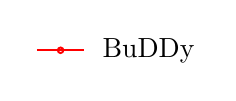
\begin{tikzpicture}
      \begin{customlegend}[
        legend columns=-1,
        legend style={draw=none,column sep=1ex},
        legend entries={BuDDy}
        ]
        \addlegendimage{style=plot_buddy}
      \end{customlegend}
    \end{tikzpicture}
    
    \caption{Running time for \emph{Tic-Tac-Toe} with $N=21$.}
  \end{figure}

\end{frame}

\begin{frame}[fragile]
  \begin{columns}
  \begin{column}{0.49\textwidth}
    \begin{figure}
      \centering

      \begin{subfigure}{1\linewidth}
        \centering

        \begin{tikzpicture}[scale=0.9, every node/.style={transform shape}]
          % blocks
          \draw[draw=gray, dashed] (-0.45,-0.45) rectangle ++(1.3,0.9);
          \draw[draw=gray, dashed] (-0.45,-2.35) rectangle ++(1.95,1.85);
          \draw[draw=gray, dashed] (-1.5,-3.32) rectangle ++(3,0.9);
          \draw[draw=gray, dashed] (-1.5,-4.35) rectangle ++(3,0.9);

          % nodes
            % nodes
  \node[shape = circle, draw = black]
  (0) {$x_0$};

  \node[shape = circle, draw = black, below right= .4cm and .5cm of 0]
  (1) {$x_1$};

  \node[shape = circle, draw = black, below left=.4cm and .5cm of 1]
  (2) {$x_2$};

  \node[shape = circle, draw = black, below left=.4cm and .5cm of 2]
  (31) {$x_3$};
  \node[shape = circle, draw = black, below right=.4cm and .5cm of 2]
  (32) {$x_3$};

  % leafs
  \node[shape = rectangle, draw = black, below=.4cm of 31]
  (sink_T) {$\top$};

  \node[shape = rectangle, draw = black, below=.4cm of 32]
  (sink_F) {$\bot$};

  % arcs
  \draw[->, dashed]
    (0)  edge (2)
    (1)  edge (2)
    (2)  edge (31)
    (31) edge (sink_T)
    (32) edge (sink_F)
  ;

  \draw[->]
    (0)  edge (1)
    (1)  edge (32)
    (2)  edge (32)
    (31) edge (sink_F)
    (32) edge (sink_T)
  ;

          % animations (nodes)
          \onslide<2>{
            \node[shape = circle, orange, draw = orange]
            {$x_0$};
          }

          \onslide<3>{
            \node[shape = circle, orange, draw = orange, below left=.4cm and .5cm of 1]
            {$x_2$};
          }

          \onslide<4>{
            \node[shape = circle, orange, draw = orange, below left=.4cm and .5cm of 2]
            {$x_3$};
          }

          \onslide<5>{
            \node[shape = rectangle, orange, draw = orange, below=.4cm of 31]
            {$\top$};
          }

          \onslide<6>{
            \node[shape = circle, orange, draw = orange, below left=.4cm and .5cm of 2]
            {$x_3$};
          }

          \onslide<7>{
            \node[shape = rectangle, orange, draw = orange, below=.4cm of 32]
            {$\bot$};
          }

          \onslide<8>{
            \node[shape = circle, orange, draw = orange, below left=.4cm and .5cm of 2]
            {$x_3$};
          }

          \onslide<9>{
            \node[shape = circle, orange, draw = orange, below left=.4cm and .5cm of 1]
            {$x_2$};
          }

          \onslide<10>{
            \node[shape = circle, orange, draw = orange, below right=.4cm and .5cm of 2]
            {$x_3$};
          }

          \onslide<11>{
            \node[shape = rectangle, orange, draw = orange, below=.4cm of 32]
            {$\bot$};
          }

          \onslide<12>{
            \node[shape = circle, orange, draw = orange, below right=.4cm and .5cm of 2]
            {$x_3$};
          }

          \onslide<13>{
            \node[shape = rectangle, orange, draw = orange, below=.4cm of 31]
            {$\top$};
          }

          \onslide<14>{
            \node[shape = circle, orange, draw = orange, below right=.4cm and .5cm of 2]
            {$x_3$};
          }

          \onslide<15>{
            \node[shape = circle, orange, draw = orange, below left=.4cm and .5cm of 1]
            {$x_2$};
          }

          \onslide<16>{
            \node[shape = circle, orange, draw = orange]
            {$x_0$};
          }

          \onslide<17>{
            \node[shape = circle, orange, draw = orange, below right= .4cm and .5cm of 0]
            {$x_1$};
          }

          \onslide<18>{
            \node[shape = circle, orange, draw = orange, below left=.4cm and .5cm of 1]
            {$x_2$};
          }

          \onslide<19>{
            \node[shape = circle, orange, draw = orange, below right= .4cm and .5cm of 0]
            {$x_1$};
          }

          \onslide<20>{
            \node[shape = circle, orange, draw = orange, below right=.4cm and .5cm of 2]
            {$x_3$};
          }

          \onslide<21>{
            \node[shape = circle, orange, draw = orange, below right= .4cm and .5cm of 0]
            {$x_1$};
          }

          \onslide<22>{
            \node[shape = circle, orange, draw = orange]
            {$x_0$};
          }

          % animations (I/Os)
          \onslide<2-3>{
            \draw[draw=purple] (-0.45,-0.45) rectangle ++(1.3,0.9);
          }
          \onslide<3-4>{
            \draw[draw=purple] (-0.45,-2.35) rectangle ++(1.95,1.85);
          }
          \onslide<4-15>{
            \draw[draw=purple] (-1.5,-3.32) rectangle ++(3,0.9);
          }
          \onslide<5-8>{
            \draw[draw=purple] (-1.5,-4.35) rectangle ++(3,0.9);
          }
          \onslide<9-10>{
            \draw[draw=purple] (-0.45,-2.35) rectangle ++(1.95,1.85);
          }
          \onslide<11-14>{
            \draw[draw=purple] (-1.5,-4.35) rectangle ++(3,0.9);
          }
          \onslide<15-22>{
            \draw[draw=purple] (-0.45,-2.35) rectangle ++(1.95,1.85);
          }
          \onslide<16-19>{
            \draw[draw=purple] (-0.45,-0.45) rectangle ++(1.3,0.9);
          }
          \onslide<20-21>{
            \draw[draw=purple] (-1.5,-3.32) rectangle ++(3,0.9);
          }
          \onslide<22>{
            \draw[draw=purple] (-0.45,-0.45) rectangle ++(1.3,0.9);
          }

          % animations (cache)
          \onslide<8->{
            \node[gray, right=.02cm of 31]
            {\tiny $1$};
          }

          \onslide<14->{
            \node[gray, left=.02cm of 32]
            {\tiny $1$};
          }

          \onslide<15->{
            \node[gray, right=.02cm of 2]
            {\tiny $2$};
          }

          \onslide<21->{
            \node[gray, left=.02cm of 1]
            {\tiny $3$};
          }

          \onslide<22-23>{
            \node[gray, right=.02cm of 0]
            {\tiny $5$};
          }
        \end{tikzpicture}

        \caption{$(x_0 \wedge x_1 \wedge x_3) \vee (x_2 \oplus x_3)$}
      \end{subfigure}

      %\caption{Blocks active in memory}
    \end{figure}

  \end{column}

  \begin{column}{0.49\textwidth}
    \begin{center}
      % { \small
      %   \begin{equation*}
      %     \texttt{cp}(n) =
      %     \begin{cases}
      %       1 & n = \top
      %       \\
      %       0 & n = \bot
      %       \\
      %       \texttt{cp}(n.low) + \texttt{cp}(n.high) & \text{otherwise}
      %     \end{cases}
      %   \end{equation*}
      % }

      % \vspace{20pt}

      $M = 4$, $B = 2$

      \vspace{10pt}

      \begin{tabular}{c c}
        node I/Os & cache lookups
        \\ \hline
        \only<1>{$0$}%
        \only<2>{$1$}%
        \only<3>{$2$}%
        \only<4>{$3$}%
        \only<5-8>{$4$}%
        \only<9-10>{$5$}%
        \only<11-14>{$6$}%
        \only<15>{$7$}%
        \only<16-19>{$8$}%
        \only<20-21>{$9$}%
        \only<22->{$10$}%
                  &
                    \only<1>{$0$}%
                    \only<2>{$1$}%
                    \only<3>{$2$}%
                    \only<4-9>{$3$}%
                    \only<10-16>{$4$}%
                    \only<17>{$5$}%
                    \only<18-19>{$6$}%
                    \only<20->{$7$}%
      \end{tabular}
    \end{center}

  \end{column}
\end{columns}

\end{frame}

\blankframe

\begin{frame}
  % Let every node be uniquely identified by a tuple $(\mathit{label},
  % \mathit{id}) : \N \times \N$.

  \begin{center}
    \begin{tikzpicture}[scale=0.9, every node/.style={transform shape}]
      \node[shape = circle, black, inner sep=6pt, draw = black] (before_n) {$x_i$};
\node[shape = circle, black, draw = black, below left=1cm and 0.4cm of before_n] (before_low) {};
\node[shape = circle, black, draw = black, below right=1cm and 0.4cm of before_n] (before_high) {};

\draw[->, dashed] (before_n) edge (before_low);
\draw[->] (before_n) edge (before_high);

% implication
\node[shape = circle, black,below right=0cm and 1.2cm of before_n] (implies) {$\implies$};

% after
\node[shape = circle, black, draw = black, right=3cm of before_n] (after_n) {\tiny $(i,\mathit{id})$};
\node[shape = circle, black, draw = black, below left=0.9cm and 0.4cm of after_n] (after_low) {};
\node[shape = circle, black, draw = black, below right=0.9cm and 0.4cm of after_n] (after_high) {};

\draw[->, dashed] (after_n) edge (after_low);
\draw[->] (after_n) edge (after_high);

    \end{tikzpicture}
  \end{center}
  % Nodes are ordered based on their \emph{uid} as follows
  \vspace{20pt}\pause
  \begin{equation*}
    \label{eq:ordering}
    (i_1, \mathit{id}_1) < (i_2, \mathit{id}_2)
    \equiv
    i_1 < i_2 \vee (i_1 = i_2 \wedge \mathit{id}_i < \mathit{id}_j)
  \end{equation*}
\end{frame}

\begin{frame}
  \begin{figure}
    \centering

    \begin{subfigure}{0.49\linewidth}
      \centering

      \begin{subfigure}[b]{0.33\linewidth}
        \centering

        \begin{tikzpicture}[scale=0.6, every node/.style={transform shape}]
            % nodes
  \node[shape = circle, draw = black]
  (0) {$x_0$};

  \node[shape = circle, draw = black, below right= .4cm and .5cm of 0]
  (1) {$x_1$};

  \node[shape = circle, draw = black, below left=.4cm and .5cm of 1]
  (2) {$x_2$};

  \node[shape = circle, draw = black, below left=.4cm and .5cm of 2]
  (31) {$x_3$};
  \node[shape = circle, draw = black, below right=.4cm and .5cm of 2]
  (32) {$x_3$};

  % leafs
  \node[shape = rectangle, draw = black, below=.4cm of 31]
  (sink_T) {$\top$};

  \node[shape = rectangle, draw = black, below=.4cm of 32]
  (sink_F) {$\bot$};

  % arcs
  \draw[->, dashed]
    (0)  edge (2)
    (1)  edge (2)
    (2)  edge (31)
    (31) edge (sink_T)
    (32) edge (sink_F)
  ;

  \draw[->]
    (0)  edge (1)
    (1)  edge (32)
    (2)  edge (32)
    (31) edge (sink_F)
    (32) edge (sink_T)
  ;
        \end{tikzpicture}
      \end{subfigure}
      \begin{subfigure}[b]{0.55\linewidth}
        \centering
        { \tiny
          \begin{tabular}{r c l}
            [ & $\triple{(0,0)}{(2,0)}{(1,0)}$ & ,
            \\ \\
              & $\triple{(1,0)}{(2,0)}{(3,1)}$ & ,
            \\ \\
              & $\triple{(2,0)}{(3,0)}{(3,1)}$ & ,
            \\ \\
              & $\triple{(3,0)}{\bot}{\top}$   & ,
            \\ \\
              & $\triple{(3,1)}{\top}{\bot}$   & ]
          \end{tabular}
          \vspace{6pt}
        }
      \end{subfigure}

      \caption{$(x_0 \wedge x_1 \wedge x_3) \vee (x_2 \oplus x_3)$}
    \end{subfigure}
    \begin{subfigure}{0.49\linewidth}
      \centering

      \begin{subfigure}[b]{0.33\linewidth}
        \centering
        \begin{tikzpicture}[scale=0.6, every node/.style={transform shape}]
            % nodes
  \node[shape = circle, draw = black]
  (0) {$x_0$};

  \node[shape = circle, draw = black, below left=1.4cm and .5cm of 0]
  (21) {$x_2$};

  \node[shape = circle, draw = black, below right=1.4cm and .5cm of 0]
  (22) {$x_2$};

  \node[shape = circle, draw = black, below right=0.4cm and .5cm of 21]
  (3) {$x_3$};

  % leafs
  \node[shape = rectangle, draw = black, below right=.4cm and .5cm of 3]
  (sink_F) {$\bot$};

  \node[shape = rectangle, draw = black, below left=.4cm and .5cm of 3]
  (sink_T) {$\top$};

  % arcs
  \draw[->, dashed]
    (0)  edge (21)
    (21) edge (sink_T)
    (22) edge (3)
    (3)  edge (sink_T)
  ;

  \draw[->]
    (0)  edge (22)
    (21) edge (3)
    (22) edge (sink_F)
    (3)  edge (sink_F)
  ;
        \end{tikzpicture}
      \end{subfigure}
      \begin{subfigure}[b]{0.55\linewidth}
        \centering
        { \tiny
          \begin{tabular}{r c l}
            [ & $((0,0), (2,0), (2,1))$ & ,
            \\ \\
              & $((2,0), \top, (3,0))$ & ,
            \\ \\
              & $((2,1), (3,0), \bot)$   & ,
            \\ \\
              & $((3,0), \top, \bot)$   & ]
          \end{tabular}
          \vspace{10pt}
        }
      \end{subfigure}

      \caption{$\neg (x_0 \ ?\ x_2 \vee x_3 \ :\ x_2 \wedge x_3)$}
    \end{subfigure}

    \caption{Node-based representation of prior shown BDDs}
  \end{figure}

\end{frame}

\begin{frame}
  \frametitle{CountPaths Example}

  \begin{columns}
  \begin{column}{0.49\textwidth}

    \begin{figure}
      \centering

      \begin{subfigure}{1\linewidth}
        \centering

        \begin{tikzpicture}[scale=0.9, every node/.style={transform shape}]
          % nodes
          \node[shape = circle, draw = black]
          (0) {\tiny $(0,0)$};

          \node[shape = circle, draw = black, below right= .3cm and .5cm of 0]
          (1) {\tiny $(1,0)$};

          \node[shape = circle, draw = black, below left=.3cm and .5cm of 1]
          (2) {\tiny $(2,0)$};

          \node[shape = circle, draw = black, below left=.3cm and .5cm of 2]
          (31) {\tiny $(3,0)$};
          \node[shape = circle, draw = black, below right=.3cm and .5cm of 2]
          (32) {\tiny $(3,1)$};

          % leafs
          \node[shape = rectangle, draw = black, below=.4cm of 31]
          (sink_T) {$\top$};

          \node[shape = rectangle, draw = black, below=.4cm of 32]
          (sink_F) {$\bot$};

          % arcs
          \draw[->,dashed]
          (0) edge (2)
          (1) edge (2)
          (2) edge (31)
          (31) edge (sink_T)
          (32) edge (sink_F)
          ;

          \draw[->]
          (0) edge (1)
          (1) edge (32)
          (2) edge (32)
          (31) edge (sink_F)
          (32) edge (sink_T)
          ;

          % animations
          \onslide<3-5>{ % 0
            \node[shape = circle, orange, draw = orange]
            {\tiny $(0,0)$};
            \draw[->,dashed,orange] (0) edge (2);
            \draw[->,orange] (0) edge (1);
          }

          \onslide<6-9>{ % 1
            \node[shape = circle, orange, draw = orange, below right= .3cm and .5cm of 0]
            {\tiny $(1,0)$};
            \draw[->,dashed,orange] (1) edge (2);
            \draw[->,orange] (1) edge (32);
          }

          \onslide<10-14>{ % 2
            \node[shape = circle, orange, draw = orange, below left=.3cm and .5cm of 1]
            {\tiny $(2,0)$};
            \draw[->,dashed,orange] (2) edge (31);
            \draw[->,orange] (2) edge (32);
          }

          \onslide<15-18>{ % 31
            \node[shape = circle, orange, draw = orange, below left=.3cm and .5cm of 2]
            {\tiny $(3,0)$};
            \draw[->,dashed,orange] (31) edge (sink_T);
            \draw[->,orange] (31) edge (sink_F);
          }

          \onslide<19-22>{ % 32
            \node[shape = circle, orange, draw = orange, below right=.3cm and .5cm of 2]
            {\tiny $(3,1)$};
            \draw[->,dashed,orange] (32) edge (sink_F);
            \draw[->,orange] (32) edge (sink_T);
          }
        \end{tikzpicture}

        \caption{\small $(x_0 \wedge x_1 \wedge x_3) \vee (x_2 \oplus x_3)$}
      \end{subfigure}

      %\caption{In-order traversal of BDD}
    \end{figure}

  \end{column}
  \begin{column}{0.49\textwidth}
    \centering

    \onslide<5->{ \small
      \begin{tabular}{c c c}
        \onslide<5-22>{\hspace{10pt}Seek\hspace{10pt}}
        \onslide<5-22>{& \hspace{10pt}Sum\hspace{10pt}}
        \onslide<5-23>{& \hspace{10pt}Result\hspace{10pt}}
        \\
        \textcolor{orange}{%
        \only<5-8>{$(1,0)$}%
        \only<9-13>{$(2,0)$}%
        \only<14-17>{$(3,0)$}%
        \only<18-22>{$(3,1)$}%
        }
        &
        % (1,0)
          \only<5-6>{$0$}%
          \only<7-8>{$1$}%
          % (2,0)
          \only<9-10>{$0$}%
          \only<11>{$1$}%
          \only<12-13>{$2$}%
          % (3,0)
          \only<14-15>{$0$}%
          \only<16-17>{$2$}%
          % (3,1)
          \only<18-19>{$0$}%
          \only<20>{$1$}%
          \only<21-22>{$3$}%
        &
          \only<1-16>{$0$}%
          \only<17-21>{$2$}%
          \only<22-23>{$5$}%
      \end{tabular}
    }

    \vspace{20pt}

    \onslide<2->{
      {\footnotesize Priority Queue: $Q_{\mathit{count}}$:

        \begin{tabular}{rll}
          [ & \onslide<4-6>{$(\arc{(0,0)}{\top}{(1,0)}, \quad 1)$  & ,}
          \\
            & \onslide<4-10>{$(\arc{(0,0)}{\bot}{(2,0)}, \quad 1)$  & ,}
          \\
            & \onslide<8-11>{$(\arc{(1,0)}{\bot}{(2,0)}, \quad 1)$  & ,}
          \\
            & \onslide<13-15>{$(\arc{(2,0)}{\bot}{(3,0)}, \quad 2)$  & ,}
          \\
            & \onslide<8-19>{$(\arc{(1,0)}{\top}{(3,1)}, \quad 1)$   & ,}
          \\
            & \onslide<13-20>{$(\arc{(2,0)}{\top}{(3,1)}, \quad 2)$ }  & ]
        \end{tabular}
      }
    }

  \end{column}
\end{columns}

\end{frame}

\begin{frame}
  \frametitle{Apply Example ($\wedge$)}

  % NOTE: The algorithm as presented here has a bug. Here, we break ties on
% 'min(t1,t2)' with 'max(t1,t2)'. Yet, this can make it unable to merge two
% paths to the same tuple (t1,t2) as intended.
%
% With Adiar v1.0.1 this was fixed by breaking ties with a lexicographical
% sorting of the tuple '(t1,t2)' instead. See the accompanying unit test for a
% counter-example.


\begin{columns}
  \begin{column}{0.24\textwidth}
    \begin{figure}
      \centering

      \begin{subfigure}{1\linewidth}
        \centering

        \begin{tikzpicture}[scale=0.5, every node/.style={transform shape}]
          % nodes
          \node[shape = circle, draw = black]
          (0) {\tiny $(0,0)$};

          \node[shape = circle, draw = black, below right= .3cm and .5cm of 0]
          (1) {\tiny $(1,0)$};

          \node[shape = circle, draw = black, below left=.3cm and .5cm of 1]
          (2) {\tiny $(2,0)$};

          \node[shape = circle, draw = black, below left=.3cm and .5cm of 2]
          (31) {\tiny $(3,0)$};
          \node[shape = circle, draw = black, below right=.3cm and .5cm of 2]
          (32) {\tiny $(3,1)$};

          % leafs
          \node[shape = rectangle, draw = black, below=.4cm of 31]
          (sink_T) {$\top$};

          \node[shape = rectangle, draw = black, below=.4cm of 32]
          (sink_F) {$\bot$};

          % arcs
          \draw[->,dashed]
          (0) edge (2)
          (1) edge (2)
          (2) edge (31)
          (31) edge (sink_T)
          (32) edge (sink_F)
          ;

          \draw[->]
          (0) edge (1)
          (1) edge (32)
          (2) edge (32)
          (31) edge (sink_F)
          (32) edge (sink_T)
          ;

          % animations
          \onslide<2-4>{ % 0
            \node[shape = circle, orange, draw = orange]
            {\tiny $(0,0)$};
            \draw[->,dashed,orange] (0) edge (2);
            \draw[->,orange] (0) edge (1);
          }

          \onslide<5-7>{ % 1
            \node[shape = circle, orange, draw = orange, below right= .3cm and .5cm of 0]
            {\tiny $(1,0)$};
            \draw[->,dashed,orange] (1) edge (2);
            \draw[->,orange] (1) edge (32);
          }

          \onslide<8-12>{ % 2
            \node[shape = circle, orange, draw = orange, below left=.3cm and .5cm of 1]
            {\tiny $(2,0)$};
            \draw[->,dashed,orange] (2) edge (31);
            \draw[->,orange] (2) edge (32);
          }

          \onslide<13-26>{ % 31
            \node[shape = circle, orange, draw = orange, below left=.3cm and .5cm of 2]
            {\tiny $(3,0)$};
            \draw[->,dashed,orange] (31) edge (sink_T);
            \draw[->,orange] (31) edge (sink_F);
          }

          \onslide<27->{ % 32
            \node[shape = circle, orange, draw = orange, below right=.3cm and .5cm of 2]
            {\tiny $(3,1)$};
            \draw[->,dashed,orange] (32) edge (sink_F);
            \draw[->,orange] (32) edge (sink_T);
          }
        \end{tikzpicture}

        \caption{\tiny $(x_0 \wedge x_1 \wedge x_3) \vee (x_2 \oplus x_3)$}
      \end{subfigure}

      \begin{subfigure}{1\linewidth}
        \centering

        \begin{tikzpicture}[scale=0.5, every node/.style={transform shape}]
          % nodes
          \node[shape = circle, draw = black]
          (0) {\tiny $(0,0)$};

          \node[shape = circle, draw = black, below left=1.2cm and .5cm of 0]
          (21) {\tiny $(2,0)$};

          \node[shape = circle, draw = black, below right=1.2cm and .5cm of 0]
          (22) {\tiny $(2,1)$};

          \node[shape = circle, draw = black, below right=0.3cm and .5cm of 21]
          (3) {\tiny $(3,0)$};

          % leafs
          \node[shape = rectangle, draw = black, below right=.4cm and .5cm of 3]
          (sink_F) {$\bot$};

          \node[shape = rectangle, draw = black, below left=.4cm and .5cm of 3]
          (sink_T) {$\top$};

          % arcs
          \draw[->, dashed]
          (0) edge (21)
          (21) edge (sink_T)
          (22) edge (3)
          (3) edge (sink_T)
          ;

          \draw[->]
          (0) edge (22)
          (21) edge (3)
          (22) edge (sink_F)
          (3) edge (sink_F)
          ;

          % animations
          \onslide<2-4>{ % 0
            \node[shape = circle, orange, draw = orange] {\tiny $(0,0)$};
            \draw[->,dashed,orange] (0) edge (21);
            \draw[->,orange] (0) edge (22);
          }

          \onslide<5-12>{ % 21
            \node[shape = circle, orange, draw = orange, below left=1.2cm and .5cm of 0]
            {\tiny $(2,0)$};
            \draw[->,dashed,orange] (21) edge (sink_T);
            \draw[->,orange] (21) edge (3);
          }

          \onslide<13-18>{ % 22
            \node[shape = circle, orange, draw = orange, below right=1.2cm and .5cm of 0]
            {\tiny $(2,1)$};
            \draw[->,dashed,orange] (22) edge (3);
            \draw[->,orange] (22) edge (sink_F);
          }

          \onslide<19->{ % 3
            \node[shape = circle, orange, draw = orange, below right=0.3cm and .5cm of 21]
            {\tiny $(3,0)$};
            \draw[->,dashed,orange] (3) edge (sink_T);
            \draw[->,orange] (3) edge (sink_F);
          }
        \end{tikzpicture}

        \caption{\tiny $\neg (x_0 \ ?\ x_2 \vee x_3 \ :\ x_2 \wedge x_3)$}
      \end{subfigure}
    \end{figure}
  \end{column}
  \begin{column}{0.4\textwidth}
    \centering

    \onslide<4-29>{\tiny Seek:

      \textcolor{orange}{%
        \only<4-7>{$\min((1,0),(2,1))$}%
        \only<8-10>{$\min((2,0),(2,0))$}%
        \only<11-12>{$\min((2,0),(2,1))$}%
        \only<13-15>{$\max((2,0),(2,1))$}%
        \only<16-18>{$\min((3,1),(2,1))$}%
        \only<19-21>{$\min((3,0),(3,0))$}%
        \only<22-23>{$\min((3,1),(3,0))$}%
        \only<24-26>{$\min((3,0),\top)$}%
        \only<27-30>{$\max((3,1),(3,0))$}%
      }
    }
    \vspace{7pt}

    \onslide<3->{ \tiny Priority Queue: $Q_{\mathit{app}:1}$:

      \begin{tabular}{rll}
        [ & \onslide<3-6>{$\arc{(0,0)}{\top}{((1,0),(2,1))}$  & ,}
        \\
          & \onslide<3-9>{$\arc{(0,0)}{\bot}{((2,0),(2,0))}$  & ,}
        \\
          & \onslide<6-11>{$\arc{(1,0)}{\bot}{((2,0),(2,1))}$ & ,}
        \\
          & \onslide<6-17>{$\arc{(1,0)}{\top}{((3,1),(2,1))}$   & ,}
        \\
          & \onslide<14-20>{$\arc{(2,1)}{\bot}{((3,0),(3,0))}$  & ,}
        \\
          & \onslide<9-22>{$\arc{(2,0)}{\top}{((3,1),(3,0))}$   & ,}
        \\
          & \onslide<17-22>{$\arc{(2,2)}{\bot}{((3,1),(3,0))}$  & ,}
        \\
          & \onslide<9-25>{$\arc{(2,0)}{\bot}{((3,0),\top)}$}   & ]
      \end{tabular}
    }

    \vspace{7pt}

    \onslide<12->{ \tiny Priority Queue: $Q_{\mathit{app}:2}$:

      \begin{tabular}{rll}
        [ & \onslide<12-14>{$\arc{(1,0)}{\bot}{((2,0),(2,1))} \quad ((3,0),(3,1))$ & ,}
        \\
          & \onslide<23-28>{$\arc{(2,0)}{\top}{((3,1),(3,0))} \quad (\top,\bot)$ & ,}
        \\
          & \onslide<23-28>{$\arc{(2,2)}{\bot}{((3,1),(3,0))} \quad (\top,\bot)$} & ]
      \end{tabular}
    }

    \vspace{7pt}

  \end{column}
  \begin{column}{0.35\textwidth}
    \centering

    \onslide<7->{ \tiny Output:

      \textcolor{blue}{%
        \only<0-7>{$\arc{(0,0)}{\top}{(1,0)}$}%
        \only<10>{$\arc{(0,0)}{\bot}{(2,0)}$}%
        \only<15>{$\arc{(1,0)}{\bot}{(2,1)}$}%
        \only<18>{$\arc{(1,0)}{\top}{(2,2)}$}%
        \only<21>{$\arc{(2,1)}{\bot}{(3,0)}$}%
        \only<26>{$\arc{(2,0)}{\bot}{(3,1)}$}%
        \only<29>{$\arc{(2,0)}{\top}{(3,2)}, \arc{(2,2)}{\bot}{(3,2)}$}%
      }%
      \textcolor{red}{%
        \only<14>{$\arc{(2,1)}{\top}{\bot}$}%
        \only<17>{$\arc{(2,2)}{\top}{\bot}$}%
        \only<20>{$\arc{(3,0)}{\bot}{\top}, \arc{(3,0)}{\top}{\bot}$}%
        \only<25>{$\arc{(3,1)}{\bot}{\top}, \arc{(3,1)}{\top}{\bot}$}%
        \only<28>{$\arc{(3,2)}{\bot}{\bot}, \arc{(3,2)}{\top}{\bot}$}%
      }%
      {% phantoms
        \only<8-9>{\phantom{$\arc{(0,0)}{\top}{(0,0)}$}}%
        \only<11-13>{\phantom{$\arc{(0,0)}{\top}{(0,0)}$}}%
        \only<16>{\phantom{$\arc{(0,0)}{\top}{(0,0)}$}}%
        \only<19>{\phantom{$\arc{(0,0)}{\top}{(0,0)}$}}%
        \only<22-24>{\phantom{$\arc{(0,0)}{\top}{(0,0)}$}}%
        \only<27>{\phantom{$\arc{(0,0)}{\top}{(0,0)}$}}%
        \only<30>{\phantom{$\arc{(0,0)}{\top}{(0,0)}$}}%
      }%
    }
    \vspace{10pt}

    \begin{tikzpicture}[scale=0.7, every node/.style={transform shape}]
      % level: 0
      % (0,0), (0,0)    1
      \onslide<3->{
        \node[shape = circle, draw = black]
        (00) {\tiny $(0,0)$};
      }

      % level: 1
      % (1,0), (2,1)    1
      \onslide<6->{
        \node[shape = circle, draw = black, below right= .5cm and .3cm of 00]
        (10) {\tiny $(1,0)$};
      }

      % level: 2
      % (2,0), (2,1)    2
      \onslide<14->{
        \node[shape = circle, draw = black, below= 1.4cm of 00]
        (21) {\tiny $(2,1)$};
      }

      % (2,0), (2,0)    1
      \onslide<9->{
        \node[shape = circle, draw = black, left= .7cm of 21]
        (20) {\tiny $(2,0)$};
      }

      % (3,1), (2,1)    3
      \onslide<17->{
        \node[shape = circle, draw = black, right= .7cm of 21]
        (22) {\tiny $(2,2)$};
      }

      % level: 3
      % (3,0), (3,0)    1
      \onslide<20->{
        \node[shape = circle, draw = black, below= .6cm of 20]
        (30) {\tiny $(3,0)$};
      }

      % (3,0), true     2
      \onslide<25->{
        \node[shape = circle, draw = black, below= .6cm of 21]
        (31) {\tiny $(3,1)$};
      }

      % (3,1), (3,0)    3
      \onslide<28->{
        \node[shape = circle, draw = black, below= .6cm of 22]
        (32) {\tiny $(3,2)$};
      }

      % leafs
      \onslide<14->{
        \node[shape = rectangle, draw = black, below right=.9cm and .5cm of 31]
        (sink_F) {$\bot$};
      }

      \onslide<20->{
        \node[shape = rectangle, draw = black, below left=.9cm and .5cm of 31]
        (sink_T) {$\top$};
      }

      % leaf arcs
      \onslide<20->{\draw[->, red, dashed] (30) edge[bend right=10] (sink_T);}
      \onslide<25->{\draw[->, red, dashed] (31) edge[bend right=10] (sink_T);}
      \onslide<28->{\draw[->, red, dashed] (32) edge[bend right=10] (sink_F);}

      \onslide<14->{\draw[->, red] (21) edge[bend left=20] (sink_F);}
      \onslide<17->{\draw[->, red] (22) edge[bend left=60] (sink_F);}
      \onslide<20->{\draw[->, red] (30) edge[bend left=10] (sink_F);}
      \onslide<25->{\draw[->, red] (31) edge[bend left=10] (sink_F);}
      \onslide<28->{\draw[->, red] (32) edge[bend left=10] (sink_F);}
      ;

      % internal arcs
      \onslide<10->{\draw[->, blue, dashed] (20) edge (00);}
      \onslide<15->{\draw[->, blue, dashed] (21) edge (10);}
      \onslide<21->{\draw[->, blue, dashed] (30) edge (21);}
      \onslide<26->{\draw[->, blue, dashed] (31) edge (20);}
      \onslide<29->{\draw[->, blue, dashed] (32) edge (22);}

      \onslide<7->{\draw[->, blue] (10) edge (00);}
      \onslide<18->{\draw[->, blue] (22) edge (10);}
      \onslide<29->{\draw[->, blue] (32) edge (20);}
    \end{tikzpicture}

    \begin{center}
      {\bf \footnotesize (c)} ~ $(a) \land (b)$
    \end{center}
  \end{column}
\end{columns}

\end{frame}

\begin{frame}
  \frametitle{Reduce Example}

  \begin{columns}
  \begin{column}{0.25\linewidth}
    \centering

    \begin{tikzpicture}[scale=0.7, every node/.style={transform shape}]
      % level: 0
      % (0,0), (0,0)    1
      \node[shape = circle, draw = black]
      (00) {\tiny $(0,0)$};

      % level: 1
      % (1,0), (2,1)    1
      \node[shape = circle, draw = black, below right= .5cm and .3cm of 00]
      (10) {\tiny $(1,0)$};

      % level: 2
      % (2,0), (2,1)    2
      \node[shape = circle, draw = black, below= 1.4cm of 00]
      (21) {\tiny $(2,1)$};

      % (2,0), (2,0)    1
      \node[shape = circle, draw = black, left= .7cm of 21]
      (20) {\tiny $(2,0)$};

      % (3,1), (2,1)    3
      \node[shape = circle, draw = black, right= .7cm of 21]
      (22) {\tiny $(2,2)$};

      % level: 3
      % (3,0), (3,0)    1
      \node[shape = circle, draw = black, below= .6cm of 20]
      (30) {\tiny $(3,0)$};

      % (3,0), true     2
      \node[shape = circle, draw = black, below= .6cm of 21]
      (31) {\tiny $(3,1)$};

      % (3,1), (3,0)    3
      \node[shape = circle, draw = black, below= .6cm of 22]
      (32) {\tiny $(3,2)$};

      % leafs
      \node[shape = rectangle, draw = black, below right=.9cm and .5cm of 31]
      (sink_F) {$\bot$};

      \node[shape = rectangle, draw = black, below left=.9cm and .5cm of 31]
      (sink_T) {$\top$};

      % leaf arcs
      \draw[->, red, dashed]
      (30) edge[bend right=10] (sink_T)
      (31) edge[bend right=10] (sink_T)
      (32) edge[bend right=10] (sink_F)
      ;

      \draw[->, red]
      (21) edge[bend left=20] (sink_F)
      (22) edge[bend left=60] (sink_F)
      (30) edge[bend left=10] (sink_F)
      (31) edge[bend left=10] (sink_F)
      (32) edge[bend left=10] (sink_F)
      ;

      % internal arcs
      \draw[->, blue, dashed]
      (20) edge (00)
      (21) edge (10)
      (30) edge (21)
      (31) edge (20)
      (32) edge (22)
      ;

      \draw[->, blue]
      (10) edge (00)
      (22) edge (10)
      (32) edge (20)
      ;

      % animations
      \onslide<2>{
        \draw[->, orange, dashed, thick] (32) edge[bend right=10] (sink_F);
        \draw[->, orange, thick] (32) edge[bend left=10] (sink_F);
      }
      \onslide<3>{
        \draw[->, orange, dashed, thick] (31) edge[bend right=10] (sink_T);
        \draw[->, orange, thick] (31) edge[bend left=10] (sink_F);
      }
      \onslide<4>{
        \draw[->, orange, dashed, thick] (30) edge[bend right=10] (sink_T);
        \draw[->, orange, thick, thick] (30) edge[bend left=10] (sink_F);
      }
      \onslide<7>{
        \draw[->, purple, dashed, thick] (32) edge (22);
        \draw[->, purple, thick] (32) edge (20);
      }
      \onslide<8>{
        \draw[->, purple, dashed, thick] (31) edge (20);
      }
      \onslide<9>{
        \draw[->, purple, dashed, thick] (30) edge (21);
      }
      \onslide<10>{
        \draw[->, orange, thick] (22) edge[bend left=60] (sink_F);
      }
      \onslide<11>{
        \draw[->, orange, thick] (21) edge[bend left=20] (sink_F);
      }
      \onslide<15>{
        \draw[->, purple, thick] (22) edge (10);
      }
      \onslide<16>{
        \draw[->, purple, dashed, thick] (21) edge (10);
      }
      \onslide<17>{
        \draw[->, purple, dashed, thick] (20) edge (00);
      }
      \onslide<20>{
        \draw[->, purple, thick] (10) edge (00);
      }
    \end{tikzpicture}

    \begin{center}
      {\bf \footnotesize (c)} ~ $(a) \land (b)$
    \end{center}
  \end{column}
  \begin{column}{0.49\linewidth}
    \centering

    \onslide<7->{ \tiny Priority Queue: $Q_{\mathit{red}}$:

      \begin{tabular}{rll}
        [ & \onslide<7-9>{$\arc{(2,2)}{\bot}{\bot}$      & ,}
        \\
          & \onslide<9-10>{$\arc{(2,1)}{\bot}{(3,\max)}$ & ,}
        \\
          & \onslide<7-11>{$\arc{(2,0)}{\top}{\bot}$     & ,}
        \\
          & \onslide<8-11>{$\arc{(2,0)}{\bot}{(3,\max)}$ & ,}
        \\
          & \onslide<15-17>{$\arc{(1,0)}{\top}{\bot}$      & ,}
        \\
          & \onslide<16-17>{$\arc{(1,0)}{\bot}{(2,\max)}$  & ,}
        \\
          & \onslide<20>{$\arc{(0,0)}{\top}{(1,\max)}$  & ,}
        \\
          & \onslide<17-20>{$\arc{(0,0)}{\bot}{(2,\max)}$} & ]
      \end{tabular}
    }

    \vspace{10pt}

    \only<2-9>{ \tiny Level: $3$

      \only<2->{
        \begin{tabular}{r>{\centering}m{3cm}l}
          [ & \onslide<2-6>{$[(3,2) \mapsto \bot]$} & ]
        \end{tabular}
      }

      \vspace{5pt}

      \onslide<3->{%
        \begin{tabular}{r>{\centering}m{3cm}l}
          [ & \only<3-4>{$\triple{(3,1)}{\top}{\bot}$}
              \only<5-7>{$[(3,1) \mapsto (3,\max)]$}
              \only<8->{\phantom{$[(3,1) \mapsto (3,\max)]$}}
          & ,
          \\
            & \only<4-5>{$\triple{(3,0)}{\top}{\bot}$}
              \only<6-8>{$[(3,0) \mapsto (3,\max)]$}
          & ]
        \end{tabular}
      }%
    }
    \only<10-17>{ \tiny Level: $2$

      \only<10->{
        \begin{tabular}{r>{\centering}m{3cm}l}
          [ & \onslide<10-14>{$[(2,2) \mapsto \bot]$} & ]
        \end{tabular}
      }

      \vspace{5pt}

      \onslide<11->{%
        \begin{tabular}{r>{\centering}m{3cm}l}
          [ & \only<11-12>{$\triple{(2,1)}{(3,\max)}{\bot}$}
              \only<13-15>{$[(2,1) \mapsto (2,\max)]$}
              \only<16->{\phantom{$[(2,1) \mapsto (2,\max)]$}}
          & ,
          \\
            & \only<12-13>{$\triple{(2,0)}{(3,\max)}{\bot}$}
              \only<14-16>{$[(2,0) \mapsto (2,\max)]$}
          & ]
        \end{tabular}
      }%
    }
    \only<18-20>{ \tiny Level: $1$

      \begin{tabular}{r>{\centering}m{3cm}l}
        [ & \phantom{$[(1,0) \mapsto \bot]$} & ]
      \end{tabular}

      \vspace{5pt}

      \begin{tabular}{r>{\centering}m{3cm}l}
        [ & \only<18>{$\triple{(1,0)}{(2,\max)}{\bot}$}
            \only<19>{$[(1,0) \mapsto (1,\max)]$}
            \only<20->{\phantom{$[(1,0) \mapsto (1,\max)]$}}
        & ]
      \end{tabular}
      \vspace{8pt}
    }
    \only<21-23>{ \tiny Level: $0$

      \begin{tabular}{r>{\centering}m{3cm}l}
        [ & \phantom{$[(1,0) \mapsto \bot]$} & ]
      \end{tabular}

      \vspace{5pt}

      \begin{tabular}{r>{\centering}m{3cm}l}
        [ & \only<21>{$\triple{(0,0)}{(2,\max)}{(1,\max)}$}
            \only<22>{$[(0,0) \mapsto (0,\max)]$}
            \only<23->{\phantom{$[(0,0) \mapsto (1,\max)]$}}
        & ]
      \end{tabular}
      \vspace{8pt}
    }

  \end{column}
  \begin{column}{0.25\linewidth}
    \centering

    \onslide<5->{ \tiny Output:

      {%
        \only<5>{$\triple{(3,\max)}{\top}{\bot}$}%
        \only<13>{$\triple{(2,\max)}{(3,\max)}{\bot}$}%
        \only<19>{$\triple{(1,\max)}{(2,\max)}{\bot}$}%
        \only<22>{$\triple{(0,\max)}{(2,\max)}{(1,\max)}$}%
      }%
      {% phantoms
        \only<-4>{\phantom{$\triple{(3,0)}{\bot}{\top}$}}%
        \only<6-12>{\phantom{$\triple{(3,0)}{\bot}{\top}$}}%
        \only<14-18>{\phantom{$\triple{(3,0)}{\bot}{\top}$}}%
        \only<20-21>{\phantom{$\triple{(3,0)}{\bot}{\top}$}}%
        \only<23->{\phantom{$\triple{(3,0)}{\bot}{\top}$}}%
      }%
    }
    \vspace{10pt}

    \begin{tikzpicture}[scale=0.7, every node/.style={transform shape}]
      % nodes
      \onslide<22->{
        \node[shape = circle, draw = black]
        (0) {\tiny $(0,\max)$};
      }

      \onslide<19->{
        \node[shape = circle, draw = black, below right= .3cm and .5cm of 0]
        (1) {\tiny $(1,\max)$};
      }

      \onslide<13->{
        \node[shape = circle, draw = black, below left=.3cm and .5cm of 1]
        (2) {\tiny $(2,\max)$};
      }

      \onslide<5->{
        \node[shape = circle, draw = black, below=.4cm of 2]
        (3) {\tiny $(3,\max)$};
      }

      \onslide<5->{
        \node[shape = rectangle, draw = black, below right=.5cm and .5cm of 3]
        (sink_F) {$\bot$};
      }

      \onslide<5->{
        \node[shape = rectangle, draw = black, below left=.5cm and .5cm of 3]
        (sink_T) {$\top$};
      }

      \onslide<5->{\draw[->, dashed] (3) edge (sink_T);}
      \onslide<13->{\draw[->, dashed] (2) edge (3);}
      \onslide<19->{\draw[->, dashed] (1) edge (2);}
      \onslide<22->{\draw[->, dashed] (0) edge (2);}

      \onslide<5->{\draw[->] (3) edge (sink_F);}
      \onslide<13->{\draw[->] (2) edge[bend left=6] (sink_F);}
      \onslide<19->{\draw[->] (1) edge (sink_F);}
      \onslide<22->{\draw[->] (0) edge (1);}
    \end{tikzpicture}

    \begin{center}
      {\bf \footnotesize (d)} ~ $(a) \land (b)$ reduced
    \end{center}
  \end{column}
\end{columns}
  
\end{frame}

\blankframe

\begin{frame}
  % same priority queue as in apply_tfp.tex

\onslide<1-15>{
  \tiny
  \begin{center}
    Levelized Priority Queue: $Q_{\mathit{app}:1}$:
  \end{center}

  \begin{center}
    \textcolor{gray}{Level: 1}
  \end{center}

  \begin{tabular}{r >{\centering}p{2.5cm}c >{\centering}p{2.5cm}c >{\centering}p{2.5cm}c >{\centering}p{2.5cm} l}
    {\normalsize [}
    & \only<2-3>{$\arc{(0,0)}{\top}{((1,0),(2,1))}$} &
                                                       {\normalsize ]}
  \end{tabular}

  \vspace{10pt}

  \begin{center}
    \textcolor{gray}{Level: 2}
  \end{center}

  \begin{tabular}{r >{\centering}p{2.5cm}c >{\centering}p{2.5cm}c >{\centering}p{2.5cm}c >{\centering}p{2.5cm} l}
    {\normalsize [}
    & \only<2-5>{$\arc{(0,0)}{\bot}{((2,0),(2,0))}$} & ,
    & \only<3-7>{$\arc{(1,0)}{\bot}{((2,0),(2,1))}$} & ,
    & \only<3-9>{$\arc{(1,0)}{\top}{((3,1),(2,1))}$} &
                                                       {\normalsize ]}
  \end{tabular}

  \vspace{10pt}

  \begin{center}
    \textcolor{gray}{Level: 3}
  \end{center}

  \begin{tabular}{r >{\centering}p{2.5cm}c >{\centering}p{2.5cm}c >{\centering}p{2.5cm}c >{\centering}p{2.5cm} l}
    {\normalsize [}
    & \only<5-10>{$\arc{(2,0)}{\bot}{((3,0),\top)}$}
      \only<11>{$\arc{(2,1)}{\bot}{((3,0),(3,0))}$} & ,
    & \only<5-12>{$\arc{(2,0)}{\top}{((3,1),(3,0))}$} & ,
    & \only<7-10>{$\arc{(2,1)}{\bot}{((3,0),(3,0))}$}
      \only<11-13>{$\arc{(2,2)}{\bot}{((3,1),(3,0))}$} & , 
    & \only<9-10>{$\arc{(2,2)}{\bot}{((3,1),(3,0))}$}
      \only<11-14>{$\arc{(2,0)}{\bot}{((3,0),\top)}$}  &
                                                         {\normalsize ]}
  \end{tabular}
}

\end{frame}

\begin{frame}
  The unique identifier of nodes and leaves can be represented in a single 64-bit
  integer.
  
  \begin{figure}
  \begin{subfigure}[b]{0.49\linewidth}
    \centering

    \begin{tikzpicture}
      \fill[black!5!white] (0,0) rectangle ++(5.4,.6);

\draw[black!60!white, pattern=north east lines, pattern color=black!30!white]
(0,0) rectangle ++(0.2,.6)
node[pos=.5]{\small\color{black} $1$};

\draw[black!60!white, pattern=north west lines, pattern color=black!30!white]
(0.2,0) rectangle ++(5,.6)
node[pos=.5]{\small\color{black} \texttt{v}};

\draw[black!60!white, pattern=north east lines, pattern color=black!30!white]
(5.2,0) rectangle ++(0.2,.6)
node[pos=.5]{\small\color{black} \texttt{f}};

    \end{tikzpicture}

    \caption{Unique identifier of a leaf \texttt{v}}
  \end{subfigure}
  \begin{subfigure}[b]{0.49\linewidth}
    \centering

    \begin{tikzpicture}
      \fill[black!5!white] (0,0) rectangle ++(5.4,.6);

\draw[black!60!white, pattern=north east lines, pattern color=black!30!white]
(0,0) rectangle ++(0.2,.6)
node[pos=.5]{\small\color{black} $1$};

\draw[black!60!white, pattern=north west lines, pattern color=black!30!white]
(0.2,0) rectangle ++(5,.6)
node[pos=.5]{\small\color{black} \texttt{v}};

\draw[black!60!white, pattern=north east lines, pattern color=black!30!white]
(5.2,0) rectangle ++(0.2,.6)
node[pos=.5]{\small\color{black} \texttt{f}};

    \end{tikzpicture}
    
    \caption{Unique identifier of an internal node}
  \end{subfigure}
  \end{figure}

  The \texttt{f} bit-flag is used to store the \emph{is\_high} boolean inside of
  the \texttt{source} of an arc.
  
\end{frame}

\begin{frame}[plain,noframenumbering]{} % like \blankframe until reveal
  \pause

  \begin{center}
    {\Huge \textbf{Adiar}}

    \vspace{12pt}
    
    \textcolor{gray}{\small
      \href{http://github.com/ssoelvsten/adiar}{github.com/ssoelvsten/adiar}
    }
  \end{center}
\end{frame}

\begin{frame}
  \begin{figure}
    \centering
    
    \begin{subfigure}[b]{0.48\linewidth}
      \centering

      \begin{tikzpicture}
        \begin{axis}[%
          width=0.95\linewidth, height=0.7\linewidth,
          every tick label/.append style={font=\scriptsize},
          % x-axis
          xlabel={number of nodes},
          xmajorgrids=true,
          xmin=51000000,
          xmax=300000000000,
          xmode = log,
          % y-axis
          ymin=1,
          ymax=1000000,
          ylabel={Time (seconds)},
          ytick distance={10},
          ymode=log,
          yminorgrids=false,
          ymajorgrids=true,
          grid style={dashed,black!20},
          ]
          \only<5-> {
            \addplot+ [style=plot_adiar]
            table {./data/queens_adiar_time.tex};
          }

          \only<2-> {
            \addplot+ [style=plot_buddy]
            table {./data/queens_buddy_time.tex};
          }

          \only<3-> {
            \addplot+ [style=plot_cudd]
            table {./data/queens_cudd_time.tex};
          }

          \only<4-> {
            \addplot+ [style=plot_sylvan]
            table {./data/queens_sylvan_time.tex};
          }
        \end{axis}
      \end{tikzpicture}

      \label{fig:queens:time}
    \end{subfigure}
    \quad
    \begin{subfigure}[b]{0.48\linewidth}
      \centering

      \begin{tikzpicture}
        \begin{axis}[%
          width=0.95\linewidth, height=0.7\linewidth,
          every tick label/.append style={font=\scriptsize},
          % x-axis
          xlabel={number of nodes},
          xmajorgrids=true,
          xmin=51000000,
          xmax=300000000000,
          xmode = log,
          % y-axis
          ymin=0,
          ymax=2.2,
          ytick distance={0.5},
          ylabel={$\mu$s / node},
          yminorgrids=true,
          ymajorgrids=true,
          grid style={dashed,black!20},
          ]

          \only<2-> {
            \addplot+ [style=plot_buddy]
            table {./data/queens_buddy_time_per_node.tex};
          }
          
          \only<3-> {
            \addplot+ [style=plot_cudd]
            table {./data/queens_cudd_time_per_node.tex};
          }

          \only<4-> {
            \addplot+ [style=plot_sylvan]
            table {./data/queens_sylvan_time_per_node.tex};
          }
          
          \only<5-> {
            \addplot+ [style=plot_adiar]
            table {./data/queens_adiar_time_per_node.tex};
          }
        \end{axis}
      \end{tikzpicture}

      \label{fig:queens:time per node}
    \end{subfigure}

    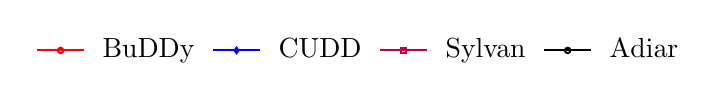
\begin{tikzpicture}
      \begin{customlegend}[
        legend columns=-1,
        legend style={draw=none,column sep=1ex},
        legend entries={BuDDy, CUDD, Sylvan, Adiar}
        ]
        \addlegendimage{style=plot_buddy}
        \addlegendimage{style=plot_cudd}
        \addlegendimage{style=plot_sylvan}
        \addlegendimage{style=plot_adiar}
      \end{customlegend}
    \end{tikzpicture}
    
    \caption{Minimum running times for the $N$-Queens problem.}
  \end{figure}

\end{frame}

\blankframe

\begin{frame}
  \begin{table}[ht!]
    \scriptsize
    
    \centering
    \begin{tabular}{r l || c | c}
      \multicolumn{2}{c||}{Algorithm} & Depth-first & Time-forwarded
      \\ \hline \hline
      Reduce         &                                    & $O(N)$                       & $O(\sort(N))$
      \\ \hline \multicolumn{4}{c}{BDD Manipulation} \\ \hline
      Apply          & $f \odot g$                        & $O(N_f \cdot N_g)$           & $O(\sort(N_f \cdot N_g))$
      \\
      If-Then-Else   & $f\ ?\ g\ :\ h$                    & $O(N_f \cdot N_g \cdot N_h)$ & $O(\sort (N_f \cdot N_g \cdot N_h))$
      \\
      Restrict       & $f|_{x_i = v}$                      & $O(N)$                       & $O(\sort(N))$
      \\
      Negation       & $\neg f$                           & $O(1)$                       & $O(1)$
      \\
      Quantification & $\exists/\forall v : f|_{x_i = v}$  & $O(N^2)$                     & $O(\sort(N^2))$
      % \\
      % \textcolor{gray}{Composition}
      %   & \textcolor{gray}{$f|_{x_i = g}$}
      %   & \textcolor{gray}{$O(N_f^2 \cdot N_g)$}
      %   & \textcolor{gray}{$O(\sort(N_f^2 \cdot N_g))$}
      \\ \hline \multicolumn{4}{c}{Counting} \\ \hline
      Count Paths    & $\# $paths in $f$ to $\top$        & $O(N)$                       & $O(\sort(N))$
      \\
      Count SAT      & $\# x : f(x)$                      & $O(N)$                       & $O(\sort(N))$
      \\ \hline \multicolumn{4}{c}{Other} \\ \hline
      Equality       & $f \equiv g$                       & $O(1)$                       & $O(\sort(N))$
      \\
      Evaluate       & $f(x)$                             & $O(L)$                       & $O(N/B)$
      \\
      Min/Max SAT    & $\min/\max\{ x \ |\ f(x) \}$       & $O(L)$                       & $O(N/B)$
    \end{tabular}

    %\caption{I/O-complexity of depth-first algorithms compared to our
    %         time-forwarded.}
  \end{table}
  
\end{frame}

\begin{frame}

  \begin{center}
    \begin{tikzpicture}[scale=0.7, every node/.style={transform shape}]
      % Main track
\node[shape = circle, draw = black, line width = 1pt] (arge) {\textbf{Arge '96}};

\node[shape = circle, draw = black, above=1cm of arge, line width = 1pt] (adiar_core) {\textbf{Adiar 1.0}};
\draw[rounded corners, line width = 3pt] (arge) -- (adiar_core);

\node[above = 3.5cm of adiar_core] (model_checking) {\color{gray} \textbf{Model Checking}};
\draw[->, gray, rounded corners, line width = 3pt] (adiar_core) -- (model_checking);

\node[above right = 1.5cm and 0.1cm of adiar_core] (equality_checking) {Equality Checking};
\draw[->, rounded corners, line width = 1.2pt] (adiar_core) |- ($(adiar_core)+(.5,2.5)$) -- (equality_checking);

\node[above left = 2.5cm and 0.1cm of adiar_core] (quantification) {Multi-variable $\exists$ / $\forall$};
\draw[->, densely dotted, rounded corners, line width = 1.2pt] (adiar_core) |- ($(adiar_core)+(-.5,3.5)$) -- (quantification);

% Tangents (mine)
\onslide<2->{
  \node[left = 4cm of adiar_core] (parallel) {\color{gray} Parallelisation};
  \draw[->, gray, rounded corners, line width = 1.2pt] (adiar_core) -- (parallel);

  \node[above left = 0cm and 1.7cm of adiar_core] (reorder) {Variable Reordering};
  \draw[->, densely dotted, rounded corners, line width = 1.2pt] (adiar_core) -- ($(adiar_core)+(-1.3,0)$) -| (reorder);

  \node[below left = 0cm and 0cm of adiar_core] (zdd) {\begin{tabular}{c} Zero-suppressed \\ Decision Diagram \end{tabular}};
  \draw[->, rounded corners, line width = 1.2pt] (adiar_core) -- ($(adiar_core)+(-1.3,0)$) -| (zdd);

  \node[above left = 0.7cm and 0cm of adiar_core] (internal) {Internal Memory};
  \draw[->, densely dotted, rounded corners, line width = 1.2pt] (adiar_core) -- ($(adiar_core)+(-1.3,0)$) -| (internal);
}

% Tangents (other)
\onslide<3->{
  \node[above right = 0cm and 1.3cm of adiar_core] (complement) {\color{gray} Attributed Edges};
  \draw[->, gray, rounded corners, line width = 1.2pt] (adiar_core) -- ($(adiar_core)+(1.3,0)$) -| (complement);

  \node[below right = 0cm and 2.3cm of adiar_core] (add) {\color{gray} \begin{tabular}{c} Arithmetic \\ Decision Diagram \end{tabular}};
  \draw[->, gray, rounded corners, line width = 1.2pt] (adiar_core) -- ($(adiar_core)+(1.3,0)$) -| (add);

  \node[right = 4.2cm of adiar_core] (proof) {\color{gray} Proof Logging};
  \draw[->, gray, rounded corners, line width = 1.2pt] (adiar_core) -- (proof);

  \node[below right = 0cm and 0.2cm of adiar_core] (verified) {\begin{tabular}{c} Formal \\ Verification \end{tabular}};
  \draw[->, densely dotted, rounded corners, line width = 1.2pt] (adiar_core) -- ($(adiar_core)+(1.3,0)$) -| (verified);
}
    \end{tikzpicture}
  \end{center}
  
\end{frame}

\end{document}

%%% Local Variables:
%%% mode: latex
%%% TeX-master: t
%%% End:
